%!TeX root = 6-perspectives.tex
\documentclass[main]{subfiles}

\begin{document}

\chapter{Toward the next generation of screenings}
\vspace*{-1\baselineskip}

\section{Limits of the Current Screening Methodologies}

As presented in our review of the different screening methodologies in the chapter 1, it is very common to screen for one particular metric whether it is the selectivity or the permselectivity or the capacity depending on the targeted application. Attempts of screening that searches for the most selective materials but combined with a good capacity are more and more common.\autocite{Chung_2019,Zhang_2022,Solanki_2020} If we take the problem of the selectivity screening, many improvements can be made in terms of calculation efficiency, or in terms of correctness of the molecular description. In the previous chapters, I mostly focused on the gain in efficiency by exploring many adsorption energy sampling techniques and by comparing their computational time as well as their accuracy. But I also started to incorporate other properties to the screening procedure by exploring the transport properties for instance. And in an effort to always aim at better efficiency, I explored alternative calculation strategies in addition to the more standard ones. 

To further improve the shortcomings of the current adsorption screening methodologies, we need to explore even more material properties. For example, the rigidity of the structures in most of the screening procedures could sometimes mislead toward materials that appear to have a very high selectivity, whereas the flexible nature of the material tend to lower the calculated selectivity. By taking into account flexibility, one could completely change the rankings found by the screening and hence finding other maybe better materials through this new approach. The other property that could completely change the results obtained by current methodologies is the polarization. For adsorbates like xenon and krypton, the difference in polarizability is in fact at the origin of the separability of these gas using an adsorbent-material. A better description of this particular property can in fact completely change the results of the screening. If we look at the best experimental materials, they are either decorated with polar groups like in the article~\cite{Li_2019} or they present open metal sites like in the article~\cite{Pei_2022}. However, we do not find these criteria as being essential when looking at the results of the current screenings. 

In this final chapter, I want to discuss three main research focuses: (i) the calculation of transport properties that could be further optimized, (ii) the adsorption calculations in flexible frameworks, and (iii) the better description of the polarization in the energy calculations.

\section{Future Developments on Transport Properties}

\subsection{Finish the optimized version of TuTraST}

Next steps in the development of the C++ tool

Layer-by-layer growth 
equivalent to find the equidistant points within $E$ and $E+\delta E$. 
Lionel Zoubritzky

\subsection{Connection to the breakthrough experiments}

Diffusion coefficients 

RUPTURA, breakthrough curve
\todo{one test with SBMOF-1 (experimental?)}
Discuss the different parameters, and their relevance.

\section{Screening flexible materials}

The reason why people usually prefer rigid frameworks is the high complexity brought by the simulation of the dynamics of a flexible framework. We already saw the cost of simulating a grand canonical ensemble using MC methods and developed strategies to avoid these type of calculations. The simulation of a flewible framework would require to relax the volume and simulate an osmotic ensemble ($\mu$,$P$,$T$), which requires MC moves on the volume of the unit cell itself.\autocite{Bousquet2012} This type of MC simulations describes more accurately every aspect of the flexibility be it the intrinsic flexibility due to thermal agitation or the adsorbate-induced flexibility. However, in a screening procedure, this type of simulation can be prohibitively long, it should however be used as an accurate method to confirm the properties of a few top materials. 

In order to incorporate flexibility effects in the screening procedure at a minimal computational cost, another approach is to use a set of rigid structures that reflects the structural diversity generated by the thermal agitation of the nanoporous material. A first study on the effect of this intrinsic flexibility on the Xe/Kr selectivity suggests that some materials could lose selectivity due to the less favorable pore size the structure vibrates.\autocite{Witman_2017} For instance, the authors explained the discrepancies between the experimental and theoretical Xe/Kr selectivity of KAXQIL\autocite{KAXQIL} by its intrinsic flexibility, which questions the performance ranking obtained by a rigid-framework screening. In this section, I will introduce in details the study of Witman et al.\autocite{Witman_2017} and I will especially focus on the case of KAXQIL presented by them. Then, I will present introduce another approach based on the structural diversity among similar deposited experimental structures. We can in fact count a dozen different structures with the same chemical nature as KAXQIL but with very different structural characteristics depending on the loaded adsorbate, which suggests an adsorbate-induced flexibility in addition to the intrinsic flexibility previously studied. 

\subsection{Snapshot method}

\subsubsection{Methodology}

To model the dynamics of the framework, Witman et al.\ use the UFF forcefield to describe the non-electrostatic framework bond potentials except for the metal bondings. For the bond dynamics around the metal, a harmonic equilibrium is fixed around the values extracted from the experimental structure. For this reason, this forcefield definition is refered to as the UFF-fix-metal (UFF-FM). In addition of the Lennard-Jones description, the point charge Coulomb interactions are described using the standard Ewald summation technique based on the charges calculated by the density derived electrostatic and chemical (DDEC) method.\autocite{manz2010chemically} Using this forcefield, the authors carried out a systematic snapshot generation of the structures from the CoRE MOF 2014 database with pre-calculated DDEC charges. And these snapshots were used to determine flexible Xe and Kr Henry constant values as well as the infinite dilution Xe/Kr selectivity. The flexible selectivity were found to be lower for {95\%} of the materials with a rigid selectivity over $25$ (as shown on the Figure~\ref{fgr:underestimated_rigid}), which suggests an over-estimation of the top performing materials. Furthermore, the effect of flexibility is much more important for the smaller pore sizes, because of the intensity of the interactions at lower distance. 

\begin{figure}[ht]
  \centering
  \begin{subfigure}[b]{0.32\textwidth}
    \centering
    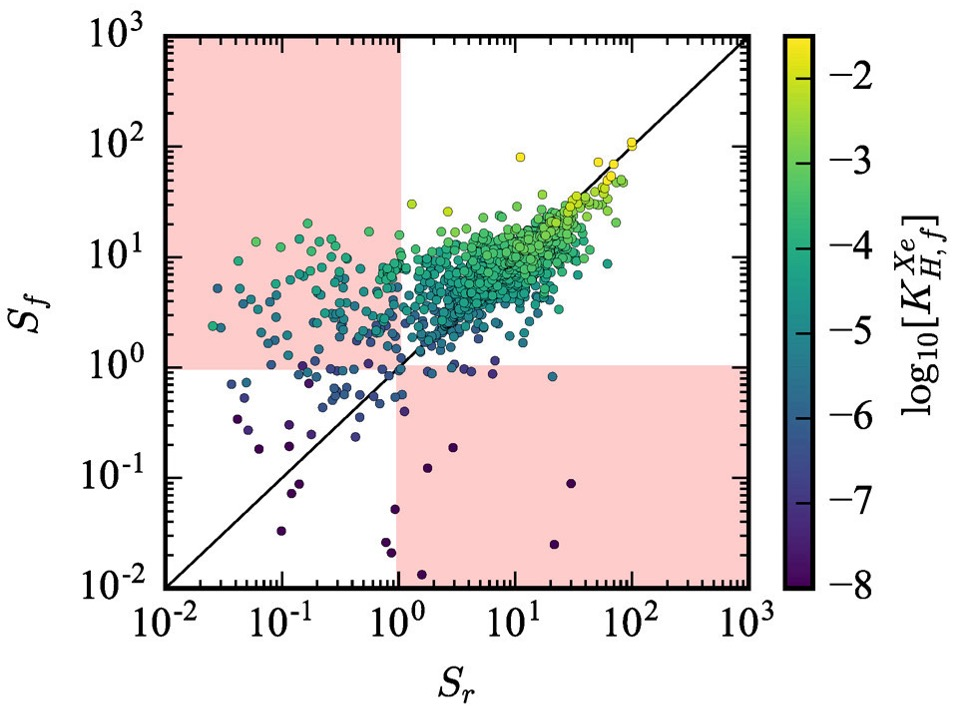
\includegraphics[width=\textwidth]{figures/6-perspectives/s_f-s_r.jpg}
    \caption{Flexible \emph{vs.} Rigid}
  \end{subfigure}
  \hfill
  \begin{subfigure}[b]{0.3\textwidth}
    \centering
    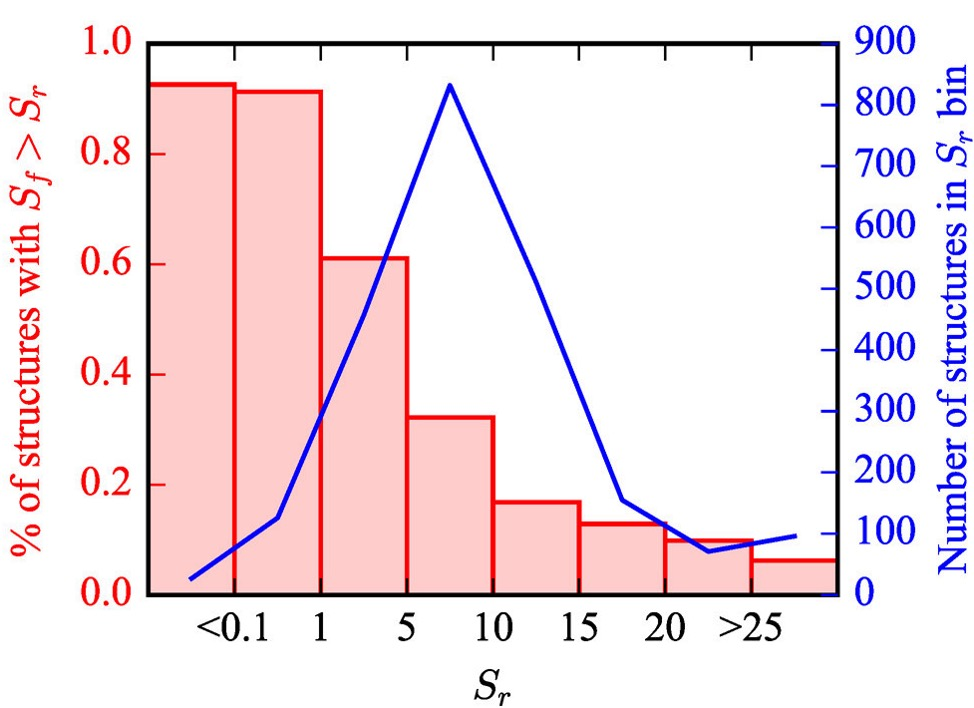
\includegraphics[width=\textwidth]{figures/6-perspectives/histogram_flex.jpg}
    \caption{selectivity underestimation}\label{fgr:underestimated_rigid}
  \end{subfigure}
  \hfill
  \begin{subfigure}[b]{0.32\textwidth}
    \centering
    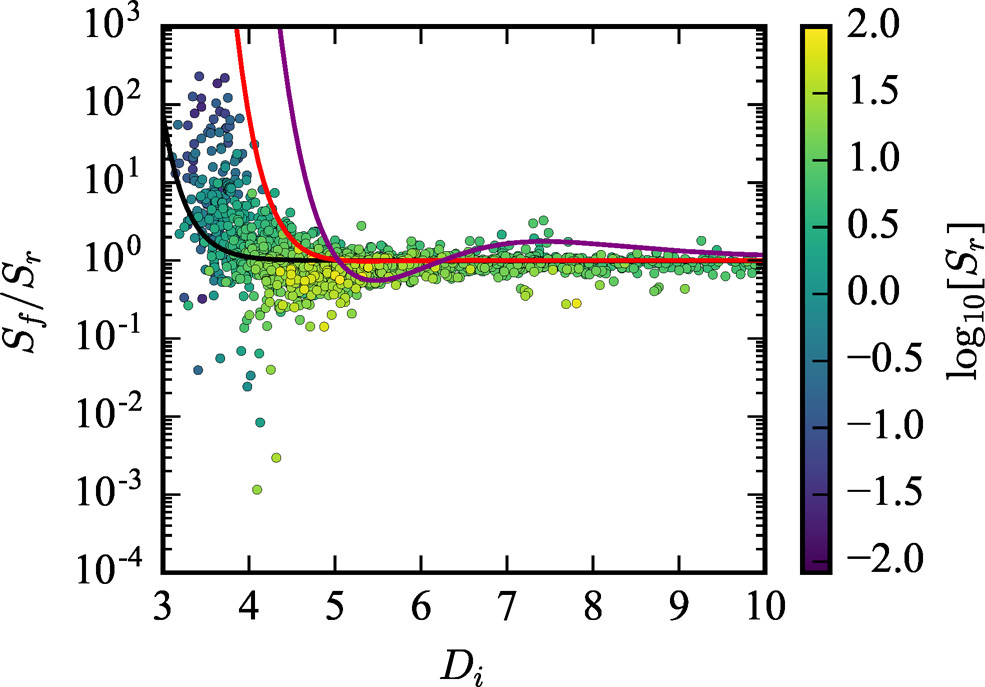
\includegraphics[width=\textwidth]{figures/6-perspectives/s_ratio_LCD.jpg}
    \caption{Flexibility effect \emph{vs.} LCD}
  \end{subfigure}
  \caption{ (a) A scatter plot of the flexible selectivity agains the rigid selectivity labeld by the log$_10$ of the flexible Xe Henry constants. (b) Barplot of the fraction of the underestimated seelctivity ($s_f>s_r$) for different categories of materials going from the least selective ones to the most selective ones ($s_r>25$). (c) Effect of the flexibility measured using the ratio $s_f/s_r$ as a funciton of the largest included sphere diameter. The line plots correspond to analytical modeling of the effect that will not be detailed here. Reprinted with permission from the original paper~\cite{Witman_2017} copyright \copyright\ 2017 American Chemical Society. }\label{fgr:flexibility_study}
\end{figure}

If we now focus on the issue of flexibility in KAXQIL, the authors used several methods to evaluate its effect on the Xe and Kr Henry constants and the Xe/Kr selectivity. For instance, they used another description of the metal--ligand bond using a cationic dummy model (UFF-CDM) and an \emph{ab initio} MD simulation using the PBE DFT function,\autocite{Perdew_1996} with a Grimme's D3 van der Waals correctio\autocite{Grimme_2010} (PBE+D3). Each of these three methods are used to generate about $30$ snapshots that were eventually used to determine the flexible framework's adsorption properties for KAXQIL.

The authors found that the lower experimental selectivity value of $16$ compared to the UFF-determined one could be partially explained by a flexibility effect. The selectivity evaluated on a rigid SBMOF-1 structure using the standard UFF forcefield is way higher than the one obtained when considering snapshots of a vibrating structure. The \emph{ab initio} MD method that should be the closest to the actual dynamics does not recover the whole phenomenon because of the system size dependence. To actually see the crystallographic deformations, multiple unit cell replications are usually necessary. Moreover, the UFF forcefield used does not give a perfect picture of the interaction energies at play in the system neither. But an overall trend is, however, drawn in this study since it is possible to attribute the discrepancies between experimental and theoretical data to the rigidity hypothesis.

\begin{table}[t]
  \centering
  \small
  \begin{tabular}{|l|c|c|c|c|}
  \hline
    Data source & Flexible &  Xe Henry Constant &  Kr Henry Constant &  Xe/Kr \\
      & structure &  \si{\mmol\per\g\per\Pa} &  \si{\mmol\per\g\per\Pa} &  selectivity \\
  \hline
    Experimental data\autocite{Banerjee_2016} & maybe &  $3.84\times 10^{-4}$ &  $2.37\times 10^{-5}$ &  $16$ \\
  \hline
    Rigid structure SBMOF-1\autocite{Banerjee_2016} & no &  $1.45\times 10^{-2}$ &  $2.70\times 10^{-4}$ &  $54$ \\
    PBE+D3 (2,2,1 unit cell) & yes &  $6.80\times 10^{-3}$ &  $1.77\times 10^{-4}$ &  $38$ \\
    UFF-FM & yes &  $6.24\times 10^{-3}$ &  $1.67\times 10^{-4}$ &  $37$ \\
    UFF-DCM & yes &  $3.18\times 10^{-3}$ &  $1.28\times 10^{-4}$ &  $25$ \\
  \hline
\end{tabular}
\caption{ Results of the flexibility analysis carried out by Witman et al., flexibility reduces the values originally calculated in a rigid structure. Reproduced with permission from the original paper~\cite{Witman_2017} copyright \copyright\ 2017 American Chemical Society.}
\label{table:witman_sbmof}
\end{table}

This approach does not give a complete picture of the flexibility effect on the selectivity value, but can rapidly identify a weakness in the rigidity hypothesis and therefore warn on a poossible over- or under-estimation of the selectivity, which can lead to identifying wrongfully a material as the best or missing the opportunity of finding a better material. The main advantage of this technique is the relative speed compared to an osmotic ensemble Monte Carlo simulation.\autocite{Bousquet2012} But the main drawback the main drawback is the imperfect description of the intrinsic flexibility as the only phenomenon at play. For instance, in the following, I will show some adsorbate-induced effects that were neglected but can be retrieved by using the multiple works on the same SBMOF-1 material. In this approach, we avoid the issues around MD simulations and we only base our reasoning on observed structural changes. 


\subsection{Experimental database approach}

According to original paper on SBMOF-1,\autocite{Banerjee_2016} the theoretical selectivity calculated by UFF is around $70.6$. However, the experimental selectivity is much lower, around $16$. To solve this mystery, Witman et al. used a snapshot-based method to evaluate the effect of selectivity. The intrinsic flexibility lowers the selectivity, which goes in the right direction to explain the difference of selectivity, but it does not seem to capture the whole picture. 

I think that the missing effect that could explain the discrepancies observed is the deformation induced by the loading of adsorbate inside the material. For instance, experimentally a structure is never empty when we resolve it by X-ray, and molecules are actually loaded inside. As shown on the Table~\ref{table:sbmof}, the structure that was originally published for its good \ce{CO2}/\ce{N2} selectivity\autocite{Yeh2012,Banerjee2012} was also tested for water adsorption, and two different structures emerged from this study: KAXQOR and KAXQIL. The first one is loaded by either air or \ce{CO2}, and the structure does not seem to be stretched as much (low LCD values around \SI{4.5}{\angstrom}). The second one, on the other hand is loaded by water that forms big clusters inside the pores and therefore stretches the pore size toward higher values (high LCD values around \SI{5.0}{\angstrom}). If we look at later studies, depending on the adsorbate (hexane, water, butane, krypton or xenon), the LCD and PLD values change in the first order according to the size of the adsorbate. There are of course other effects, like the clustering we mentioned for water, but also less expected effects such as the orientation of the adsorbate inside the structure. 

\begin{table}[t]
\centering
\setlength\extrarowheight{2pt}
\small
\begin{tabular}{|l|r|c|c|c|c|}
  \hline
  Experimental structure & Adsorbate in &  Selectivity &  LCD (\SI{}{\angstrom}) &  PLD (\SI{}{\angstrom}) &  Xe Diff. \\
  CCSD ref. code & the structure &  $s\ex{Xe/Kr}_0$ &   &   & Coeff. \si{\square\cm\per\s} \\
  \hline
  KAXQOR01\autocite{Yeh2012} & Not specified & 101 & 4,99 & 3,66 & 3$\times$10\ex{-09} \\
  KAXQOR\autocite{Banerjee2012} & Not specified & 22 & 4,51 & 4,04 & 7$\times$10\ex{-06}  \\
  KAXQIL\autocite{Banerjee2012} & H$_2$O & 104 & 5,12 & 3,77 & 3$\times$10\ex{-08} \\
  QUXRIM\autocite{Banerjee2016hydro} & hexane &  52 & 4,75 & 4,31 & 3$\times$10\ex{-05}  \\
  QUXRUY\autocite{Banerjee2016hydro} & hexane &  96 & 4,91 & 3,57 & 9$\times$10\ex{-10} \\
  QUXROS\autocite{Banerjee2016hydro} & hexane &  99 & 5,00 & 3,66 & 5$\times$10\ex{-09}  \\
  QUXREI\autocite{Banerjee2016hydro} & hexane & 101 & 5,02 & 3,67 & 7$\times$10\ex{-09}  \\
  QUXRAE\autocite{Banerjee2016hydro} & hexane & 100 & 5,03 & 3,68 & 7$\times$10\ex{-09}  \\
  QUXQUX\autocite{Banerjee2016hydro} & butane & 103 & 5,17 & 3,83 & 1$\times$10\ex{-07}   \\
  QUWYEO\autocite{Banerjee2016hydro} & butane & 100 & 4,99 & 3,65 & 5$\times$10\ex{-09} \\
  \hline  
  UQEFAZ\autocite{Banerjee_2016} & krypton & 23 & 4,53 & 4,08 & 5$\times$10\ex{-06}   \\
  UQEFED\autocite{Banerjee_2016} & xenon & 63 & 4,89 & 3,54 & 1$\times$10\ex{-11}   \\
  \hline
  \end{tabular}
  \caption{ \todo{add Henry} Structural, adsorption and transport properties of structures in the CSD database that are similar to the à SBMOF-1 structure.\autocite{Banerjee_2016} for Xe/Kr separation. The last structures actually correspond to the structures resolved in the paper presenting SBMOF-1 in Nature Communications. We can note the structural diversity that induces this diversity of properties. (The pore sizes are calculated using the CCDC radii definition.) }
  \label{table:sbmof}
\end{table}

As shown on the Figure~\ref{fgr:ads_config}, the orientation of the hexane molecule inside the material seems to favor either a configuration with a large LCD and a low PLD (QUXRUY), or a slightly lower LCD with a slightly higher PLD (QUXRIM). The material configurations are, however, a bit different from the ones observed with KXQOR or KAXQIL. 

\begin{figure}[ht]
  \centering
  \begin{subfigure}[b]{0.45\textwidth}
    \centering
    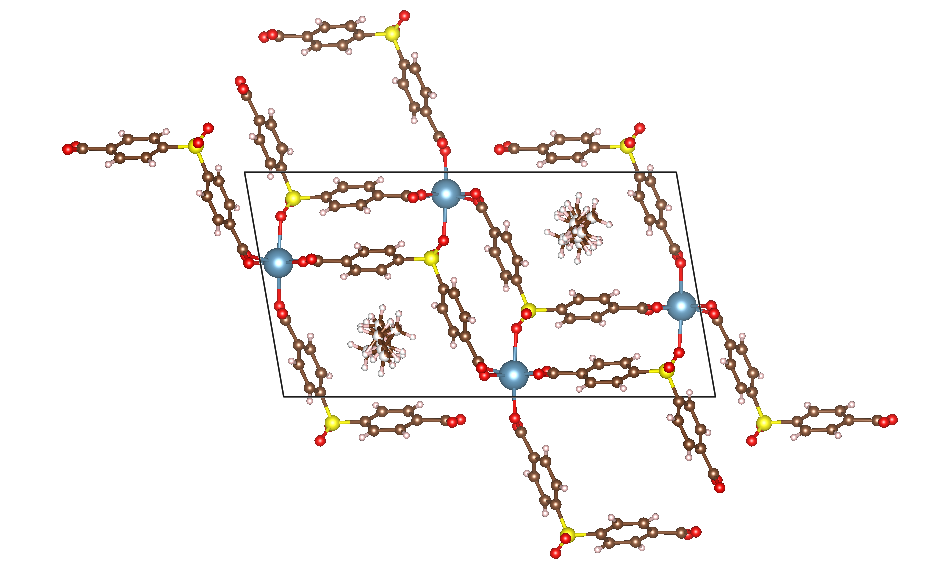
\includegraphics[height=0.6\textwidth]{figures/6-perspectives/QUXRIM.png}
    \caption{QUXRIM}\label{fgr:QUXRIM}
  \end{subfigure}
  \hfill
  \begin{subfigure}[b]{0.45\textwidth}
    \centering
    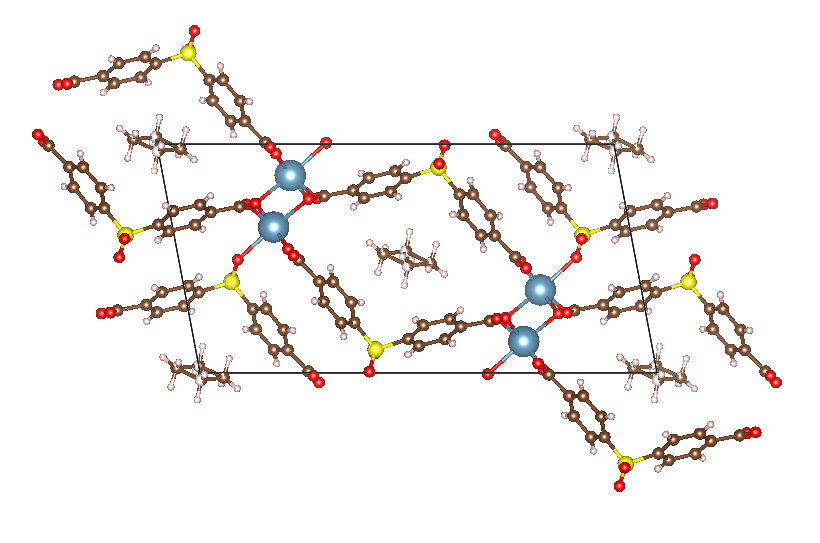
\includegraphics[height=0.6\textwidth]{figures/6-perspectives/QUXRUY.png}
    \caption{QUXRUY}\label{fgr:QUXRUY}
  \end{subfigure}
  \caption{ An illustration of the effect of the orientation of hexane inside a SBMOF-1-like material. In QUXRIM (a), the carbon atoms are oriented toward the S atoms, whereas in QUXRUY (b) they are oriented toward the Ca atoms. This difference in the orientation could explain the different structural properties of the materials reported on the Table~\ref{table:sbmof}.}\label{fgr:ads_config}
\end{figure}

Now that I characterized the adsorbate effect on a few example-configurations, we can better understand the thought process that lead to the identification of KAXQIL as a candidate for Xe/Kr separation. The KAXQIL structure is actually representing the material loaded by water with large pores which enables a good interaction with a large molecule like xenon. For this reason, it was identified as a top selective material. However, when it was experimentally tested for low pressure adsorption using the Henry constant, it is most likely that the pores are not stretched, which gave lower Henry constants than expected. The structures UQEFAZ or KAXQOR seem to a better description of this low-pressure case since the experimental selectivity values are much more consistent with their theoretical selectivity values. 

To confirm this hypothesis, we would need to measure a high-loading Xe/Kr binary mixture adsorption uptake. If xenon is highly represented in the adsorbent material, then the structure would we much more favorable to the xenon adsorption, hence increasing the selectivity value closer to the theoretically predicted one. This also highlights a composition effect, if the initial mixture has a low xenon content, the structure would most likely have narrower pores, which could decrease the selectivity. By changing the composition of the binary mixture, this effect could also be measured experimentally, if the initial hypothesis on the adsorbate-induced flexibility is correct.

This method could be used on other materials by screening for materials with a similar chemical composition and topology, for example. However, due to the bias in research focus, it not always possible to find structures in very different adsoption conditions. To work around these limitations, one could either expertimentally generate these structures when a material seems interesting to see if the flexibility plays a role in the adsorption process. Or alternatively, one could computationally generate these structures by running structure optimizations on loaded structures. Either way, this new approach to flexibility seems complementary to the ones mentioned previously because it seems to have a similar (or slightly higher due to the adsorbate) computational cost as the Witman approach, while avoiding the computationally prohibitive calculation (in a screening) presented by Bousquet et al. 


\subsubsection{Diffusion in a flexible environment}

D'autre part, le cas de UQEFED, qui représente la structure de SBMOF-1 adsorbé par du xénon déterminée par Banerjee \emph{et al.},\autocite{Banerjee_2016} allie une forte sélectivité (63) mais avec une très faible diffusivité (1$\times$10\ex{-11} \si{\square\cm\per\s}). Bien que la sélectivité thermodynamique est très bonne, cet équilibre ne peut être atteint que très lentement car les molécules de xénon n'ont pas le temps de se déplacer dans la structure. Ainsi, ce blocage cinétique pourrait également expliquer que l'expérience note des valeurs de sélectivités en décalage avec la théorie. En effet, rien ne nous dit que l'équilibre est atteint lors du tracé des isothermes expérimentales. Une pénétration lente du xénon à l'intérieur du matériau donnerait des quantités de xénon adsorbées plus faibles que prévu par la thermodynamique, ce qui mettrait en défaut les simulations théoriques. 

Fort de ces deux constats, il est plus probable que le matériau SBMOF-1 réel ait une certaine flexibilité permettant le déplacement du xénon quand les sites ne sont pas déjà occupés par du xénon. Mais lorsqu'il y a un xénon qui occupe le site, les canaux deviennent plus étroits et induisent un blocage cinétique. Ces phénomènes ne pourraient pas être révélés par une étude purement thermodynamique et montrent l'intérêt de tenir en compte de propriétés clés comme la cinétique ou la flexibilité. C'est pourquoi, il est maintenant crucial d'aller au-delà des méthodes de screening standard décrites dans la littérature et d'essayer de prendre en compte d'autres phénomènes physiques dans le screening. En considérant la flexibilité et les effets de transport on peut ainsi identifier des matériaux qui garderont leur performance lors de l'expérimentation.



\section{Noble Gas Polarizability}

\subsection{Problem definition}

\todo{put graph comparing experiment and UFF}

The beginning of some explication

Best materials use polarization effects \autocite{Li_2019,Pei_2022}

Talk about the order of magnitude of the different interactions > charge--(induced dipole high magnitude)

Standard methods failing to describe oms\autocite{Perry_2014} 

\todo{faire référence à 2-thermo partie sur les interactions\ref{sct:interaction}}

\subsubsection{Coupling with transport properties}

% Outre l'exemple très parlant de SBMOF-1, d'autres publications, dans la séparation d'hydrocarbures notamment, s'intéressent aux éventuelles blocages cinétiques grâce à des simulations de dynamique moléculaire (MD) flexible.\cite{Stanton_2022} Ils ont notamment mis en évidence que la diffusion pouvait détériorer les performances de structure présentant d'excellente performance thermodynamique (énergie d'adsorption). Cette approche est très complète, car elle allie la thermodynamique, la flexibilité et les effets de transport dans une seule étude. En revanche, elle est très coûteuse en temps de calcul et ne pourrait être appliquée qu'à une poignée de structures. Au lieu d'utiliser des champs de force flexible qui alourdissent énormément la simulation, il est possible de se tourner vers une approche en ``snapshot'' bien moins coûteuse que nous développerons dans la dernière partie de ce rapport. Dans cette partie, nous nous focaliserons uniquement sur le couplage thermodynamique/cinétique.

\subsection{Studying the polarization}

Inspired by works on the subject\autocite{Lachet_1998,Becker_2017} 

\todo{essayer d'ajouter la polarisabilité pour PEI et al. et Li et al.}

Xe/Kr difference of polarisability
Open Metal Sites/polar groups
\todo{20220421\_pres}

\todo{Not the best material, but interesting discussion on open metal site effect}
Tao et al.\autocite{Tao_2020} looked at tuning (and improving) the selective adsorption of Xe over Kr by MOF open metal sites in the UTSA-74 framework structure.



PSA for separation most commonly used: selectivity, working capacity, regenerability (kinetics and energy used to regenerate the material i.e. empty the pores for another cycle).\autocite{Kumar_1994}

\OnlyInSubfile{\printglobalbibliography}

\end{document}
